%%% Comment:
%\documentclass[english]{article}
%\usepackage[T1]{fontenc}
%\usepackage[latin9]{inputenc}
%\usepackage{babel}
%\usepackage{pdfpages}
%\usepackage{float}
%\usepackage{graphicx}
%\usepackage{mathtools}
%\usepackage[margin=0.5in]{geometry}
%\begin{document}
%
%\title{Sensors and Actuators}
%
%
%\author{David Hanley and Hong-Bin Yoon}
%
%\maketitle

\section{Summary}
Listed in this report is a set of sensors, actuators, and thrusters that could potentially be used on Cubesats from 1U to 3U. There is a wide range of sensors and actuators available for use depending on size, weight, and performance constraints. While thrusters currently on the market are generally of a lower technology readiness level than the available sensors on the market, there are still a range of options among available thrusters to choose based on size, weight, and performance constraints as well. 

Additionally, there are several integrated attitude determination and attitude control products available on the market. These systems usually are quite compact and contain star trackers, sun sensors, and reaction wheels among other sensors and actuators. Finally, the end of this report presents a short list of general suppliers that can be considered in the future for sensor and actuator parts as well as parts for other systems on the cubesat. 

\section{Inertial Measurement Unit(IMU)}

%% IMU(gyro, accelero, magneto, baro..etc)
Most Inertial Measurement Unit(IMU) or Inertial Navigation System(INS) include sensors for both position estimation and attitude estimation. \\\\

%%Silicon Sensing IMU

\begin{figure}[h!]
   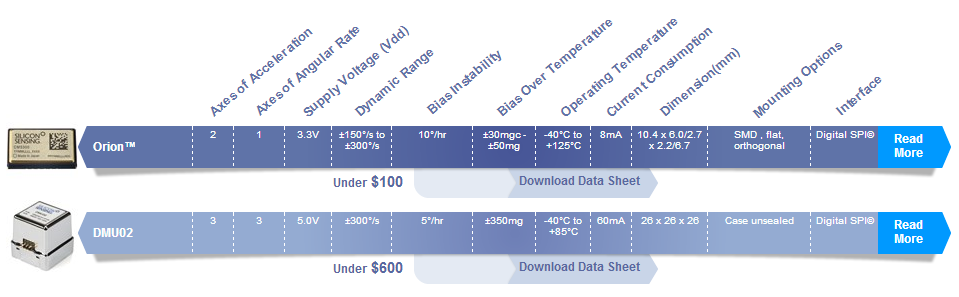
\includegraphics[scale=0.6]{../IMU/siliconSensing_IMU}
   \caption{IMU's from Silicon Sensing \cite{imu1}}
\end{figure}


%% Analog Devices IMU + Gyro + accelo
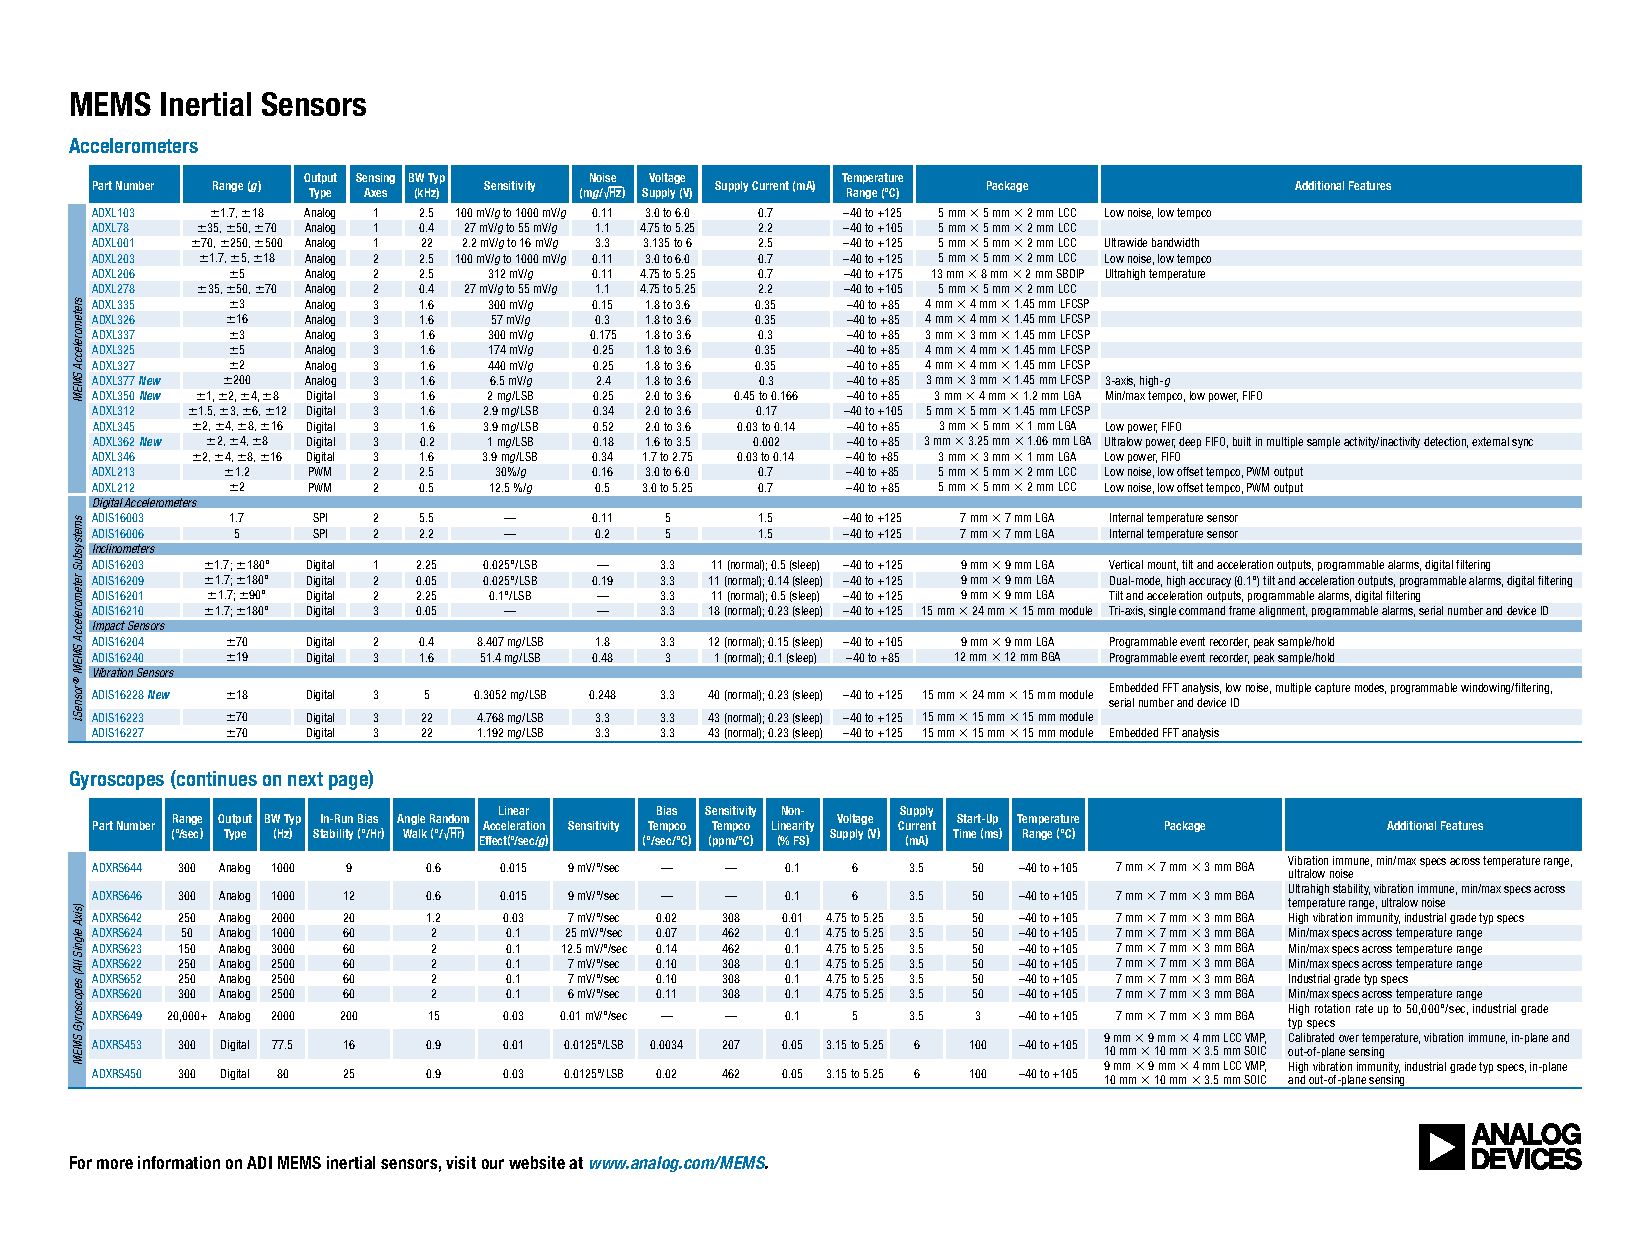
\includepdf[pages={1,2}]{../IMU/AnalogDevices_Full_List.pdf}
Information from \cite{imu2}.

\section{Position Estimation Sensors}
%% List GPS
\begin{center}

     \begin{tabular}{ |p{2cm} | p{1cm} | p{2cm} | l | l | l | p{5cm} |}
     \hline

      {\bf Name} & {\bf Mass} & {\bf Size} & {\bf Accuracy} & {\bf Type} & {\bf TRL} & {\bf Comment}  \\ \hline

     Aerocube-4 GPS \cite{Gangestad} & NA & NA &  {$ \pm 20 $} & GPS receiver & NA & Orbit determination once per day or as power system permits \\ \hline

     Nano Star Tracker on Chip (STC) \cite{Prokhorov} & 65 g & 73.5x 57.0x 57.8 mm & 10''~50'' & Star Tracker & NA & 19.5 deg field of view, update rate 10 Hz, mean power (without Peltier cooler 250mW), peak power 1 W \\ \hline
     \end{tabular}
\end{center}

\section{Attitude Estimation Sensors}
%% List Star Trackers and Sun, Earth sensors, magnetometer.

\begin{center}
     \begin{tabular}{ | p{2cm} | p{1.25cm} | p{2cm} | l | l | l | p{2cm} |}
     \hline

      {\bf Name} & {\bf Mass} & {\bf Size} & {\bf Accuracy} & {\bf Type} & {\bf TRL} & {\bf Comment}  \\ \hline

     Blue Canyon Technologies Nano Star Camera 1 \cite{BCT} & <0.5 Kg& < 5x5x10cm& 7-24 arc-sec & Star Tracker & NA & <0.5W power consumption \\ \hline

     SD085-23-21-021 \cite{aes2} & NA & 3.76x 1.5x 3.3 mm & NA & Sun Sensor & 9 & \\ \hline

     Melexis MLX90615 \cite{aes3} & NA & 4.7x 4.7x 2.7 mm& 0.5 deg over 0 to 50 deg C & Earth Nadir Sensor & 9 &  \\
     \hline

     Honeywell HMC6042 \cite{aes4} & NA & 5 x 3.6 x 1.0mm & 0.15 milliGauss & 2-Axis Magnet & 9 &   \\ \hline

     Honeywell HMC1041Z \cite{aes5} & NA &1.15x4x1.25 mm & 0.15 milliGauss & 1-Axis Magnet & 9 &   \\ \hline
     
     Space Micro Coarse Sun Sensor \cite{SMI} &  10 g & 1.27 cm diameter x0.90 cm height & 5 deg of 1 axis knowledge & Sun Sensor & 9 & \\ \hline
     
     Space Micro Medium Sun Sensor \cite{SMI} & 36 g &	2.43 cm diameter x 3.49cm height & 1 deg of 2 axis knowledge & Sun Sensor & 9 & \\ \hline
     
	Berlin Space Technologies ST-200 \cite{BST} & 50 g & 30 mm x 30 mm x 38.1 mm & 30 arc-sec (pitch/yaw), 200 arc-sec (roll) & Star Tracker & 7 & \\ \hline

	Digital Fine Sun Sensor CubeSatShop \cite{CubeShop} & 35 g & 34 mm x 32 mm x 21 mm & 0.1 deg & Sun Sensor & 7 & \\ \hline
	
	Magnetometer \cite{CubeShop} & 15 g sensor, 150 g electronics & Sensor: 10x10x5 mm, Electronics: 90x30x11 mm & Sensitivity: 10 nT & Magnetometer & 9 & \\ \hline
	
	CubeSat Sun Sensor \cite{CubeShop} & < 5 g & 33 mm x 11 mm x 6 mm & < 0.5 deg & Sun Sensor & 7 & \\ \hline

     \end{tabular}
\end{center}

\section{Inter-satellite Distance Sensors}
%% Vision and more...


\begin{center}
     \begin{tabular}{ |p{2cm} | l | l | l | l | l | p{5cm} |}
     \hline

      {\bf Name} & {\bf Mass} & {\bf Size} & {\bf Accuracy} & {\bf Type} & {\bf TRL} & {\bf Comment}  \\ \hline

     Nexus S \cite{Ref:ids2} & 129g & 123.9x 63x 11 & 1.53m , 3 deg @30 m & Vision & -  &   \\ \hline

     IBIS4-1300 \cite{Ref:ids1} & Mass & Size & < 100 arc-s & Vision & TRL & Vision based Star Tracker and Topology (for formation flying). Does not talk about satellite detection methods \\ \hline
     \end{tabular}
\end{center}


\section{Actuators}

Reaction Wheels, Extending Wings, and Integrated Packages\\


\begin{center}
     \begin{tabular}{ | p{2cm} | p{1.25cm} | p{2cm} | l | l | l | p{2cm} |}
     \hline
      {\bf Name} & {\bf Mass} & {\bf Size} & {\bf Accuracy} & {\bf Type} & {\bf TRL} & {\bf Comment}  \\ \hline
      
	  Aerocube-4 Retractable wings \cite{Gangestad} & NA & 2 wings, each 9x10cm & N/A & Extending Wings & 7 & Uses wings to adjust in-track formation for 3 satellites \\ \hline
	  
	  Blue Canyon Technologies Micro Reaction Wheel \cite{BCT} & 150 g & 43x43x18 mm & NA & Reaction Wheel & NA & Momentum: 18 mNms, Max Speed: 6000 RPM, Torque: 0.6mNm, Lifetime: > 3 years, Nominal power consumption: < 0.1W, Peak power: < 1.0W, Op Voltage: 5 to 15 V \\ \hline
	  
	  BCT Integrated Attitude Control for Cubesats \cite{BCT} & < 0.7 Kg & < 10x10x5 cm (0.5U) & Spacecraft Pointing Accuracy: 0.003 deg (1-sig) for 2 axes, 0.007 deg (1-sig) for 3rd axis	Integration Package & NA & Spacecraft Lifetime > 1 year, Nominal Power consumption: <0.5 W, Peak Power: <2.0W, Slew Rate (8kg, 3U CubeSat): > 10 deg/sec \\ \hline
	  
	  Sinclair Interplanetary RW-0.007-4 \cite{Sinclair} & 90 g & 50 mm x 40 mm x 27 mm & NA & Reaction Wheel & 7 & Nominal Torque 1 mNm, Nominal Momentum 7 mNm-sec, Supply Power 0.1 W to 0.7 W \\ \hline
	  
	   Sinclair Interplanetary RW-0.01-4 \cite{Sinclair} & 120 g & 50 mm x 50 mm x 30 mm & NA & Reaction Wheel & 7 & Nominal Torque 1 mNm, Nominal Momentum 10 mNm-sec, Supply Power 0.1 W to 0.7 W \\ \hline
	   
	   Sinclair Interplanetary RW-0.03-4 \cite{Sinclair} & 185 g & 50 mm x 50 mm x 40 mm & NA & Reaction Wheel & 9 & Nominal Torque 2 mNm, Nominal Momentum 30 mNm-sec, Supply Power 0.1 W to 1.5 W \\ \hline
	   
	   Berlin Space Technologies iACDS-100 \cite{BST} & 250 g & 95 mm x90mm x 32mm & <<1 deg pointing , (30 arc-sec in Pitch/Yaw, and 200 arcsec in Roll for att. Determination) & Integrated ACDS product & 6 & Power (Nom/Peak): 0.5W/1.8W, Actuators: 3 Reaction Wheels, 3 Magnetorquer, Sensors: Star Tracker, 3-Axes MEMS Gyro, Magnetometer, Accelerometer \\ \hline
	   
	   MAI-400 ADACS CubeSatShop \cite{CubeShop} & 694 g & 10 cm x 10 cm x 5 cm	& Integrated ACDS product & 7 & Sensors: 3-axis magnetometer, coarse sun sensor, EHS camera, Actuators: 3 torque rods \\ \hline
	   
	   MAI-300 Single Axis Reaction Wheel \cite{CubeShop} & 317 g & 68.5mm x 68.5mm x 33.0mm & NA & Reaction Wheel & 7 & Max Torque: 0.625 mNm \\ \hline
	   
	   MAI-201 Miniature 3-Axis Reaction Wheel \cite{CubeShop} & 640 g & 76.2mm x 76.2mm x 70mm & NA & Reaction Wheel & 7 & Max Torque: 0.625 mNm \\ \hline
	   
	   MAI-200 ADACS \cite{CubeShop} & 907 g & 100mm x 100mm x 78.75mm & NA & Integrated ACDS product & 7 & Max Torque: 0.625 mNm \\ \hline
     \end{tabular}
\end{center}

Magnetorquers\\

\begin{center}
     \begin{tabular}{ |p{2cm} | p{1cm} | p{1cm} |  p{1cm} | l | p{2cm} | l | p{4cm} | p{1cm} | p{3cm} |  }
     \hline

      {\bf Name} & {\bf Mass} & {\bf Size} & {\bf Accuracy} & {\bf Type} & {\bf TRL} & {\bf Comment}  \\ \hline
      
       Clyde Z-Axis Magnetorquer & 50 g & 100 x 100 x 4.3 mm & NA & Torquer & NA & magnetic moment of 0.19Am2 \\ \hline
       
	   SSBV magnetorquer rod & <30 g & L7 x D9 & NA & Torquer & NA & Magnetic moment: >0.2Am2 \\ \hline
	   
	   CubeSat Magnetorquer Rod \cite{CubeShop} & 30 g & Length 7 cm, Diameter < 9 mm & NA & Torquer & NA & Magnetic moment: 0.2 $Am^2$ \\ \hline
	   
	   CubeTorquer \cite{CubeShop} & 22.25 g & Length 60 mm, Diameter 10 mm & NA & Torquer & NA & Magnetic moment: 0.2 $Am^2$ \\ \hline
     \end{tabular}
\end{center}

\section{Thrusters}

{\bf COTS}
\begin{center}
     \begin{tabular}{ |p{2cm} | p{1cm} | p{1cm} |  p{1cm} | l | p{2cm} | l | p{4cm} | p{1cm} | p{3cm} |  }
     \hline

       {\bf Name} & {\bf Mass} & {\bf Size} & {\bf Isp} & {\bf $\Delta V$} & {\bf Thrust} & {\bf System Power}&{\bf Comment}  \\ \hline


     Spence Pressure-fed electrospray \cite{Spence} & <1.15 Kg& 0.56 U& 800 & 151 m/s & 0.7 mN &< 9W &   \\ \hline

     Micro-pulsed plasma thruster \cite{Spence} & <0.55 Kg& 0.5 U & 700 & 63 m/s&  & 2W @ 2hz fire &  Impulse: 0.5 mN-s primary, 0.13 mN-s ACS\\ \hline

     Unpressurized (wicking feed) electrospray \cite{Spence} & <0.4 Kg& 0.4 U& 750 & 76 m/s & 0.1 mN & 1W &  \\
     \hline

     Microresistojet (MRJ) \cite{Spence} & < 1.25 Kg& 1.0 U&150 & 60m/s & 2-10mN & 3-15W&   \\
     \hline

     RF Ion \cite{Spence} & <1.25 Kg& 1.25 U& 1800 & 244m/s & 0.067 mN &10W &   \\
     \hline

     Green monopropellant \cite{Spence} & < 1 Kg& 0.5 U& 240 & 130m/s & 0.5N & 15W&   \\
     \hline

	Nanosatellite Micropropulsion System \cite{Spence} & 300 g & NA &	50s-100s & NA & nominal: 100 uN to 10 mN & < 2 W & Pointing Res: 0.1 arcsec \\ \hline

     \end{tabular}
\end{center}


{\bf Not COTS}
\begin{center}
     \begin{tabular}{ |p{2cm} | p{1cm} | p{1cm} |  p{1cm} | l | l | l | p{5cm} | p{1cm} | p{2cm} |  }
     \hline

       {\bf Name} & {\bf Mass} & {\bf Size} & {\bf Isp} & {\bf $\delta V$} & {\bf Thrust} & {\bf System Power}&{\bf Comment}  \\ \hline

     Ion electrospray \cite{Ref:thr9} & & 1/3 U & 2500 & 200m/s & 0.1 mN& & \\ \hline
     {$\mu$}VAT&150g& 40x 40x 40mm & 1000&   & 5.4{$\mu$}N& & turn 90 degrees in 10 minutes. .\\ \hline
     YUsend-1 SPT \cite{Ref:thr10} &94 g &   &   &   & 0.15 mN& & \\ \hline
     \end{tabular}
\end{center}



\section{Potential Suppliers}
Blue Canyon Technologies\\
Melexis\\
Analog Devices\\
Silicon Sensing\\
Sinclair Interplanetary\\
Berlin Space Technologies\\

\bibliographystyle{IEEEtran}
\bibliography{Sensors_and_Actuators_Table}

\end{document}
